\documentclass[a4paper]{article}
\usepackage{amsmath}
\usepackage{amsfonts}
\usepackage{amssymb}
\usepackage[utf8]{inputenc}
\usepackage[T1]{fontenc}
\usepackage{graphicx}
\usepackage{hyperref}
\usepackage{tcolorbox}
\usepackage{CJKutf8}
\usepackage{tikz}

\usetikzlibrary{arrows}

\begin{document}
\begin{CJK}{UTF8}{min}
\begin{center}
{\Large\bfseries TikZ Test }\\[1em]
\end{center}
\vspace{2em}

\section*{TikZ Basic Shape Test}


\noindent 以下はTikZを使用して描画した円です。


\begin{figure}[h]
    \centering
    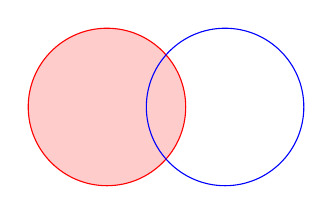
\begin{tikzpicture}

        \draw[red, fill=red!20] (0,0) circle (1cm);
        \draw[blue] (1.5,0) circle (1cm);
        
\end{tikzpicture}
    \caption{TikZ Circle}
    \label{fig:circle}
\end{figure}

\section*{TikZ Library Test}


\noindent 以下はarrowsライブラリを使用した矢印です。


\begin{figure}[h]
    \centering
    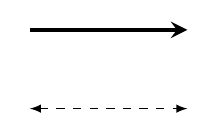
\begin{tikzpicture}

        \draw[>=stealth, ->, ultra thick] (0,0) -- (2,0);
        \draw[>=latex, <->, dashed] (0,-1) -- (2,-1);
        
\end{tikzpicture}
    \caption{TikZ Arrows}
\end{figure}

\section*{Inline TikZ Test}


\noindent 文中に


{\centering

\begin{tikzpicture}
\draw[fill=green] (0,0) circle (2pt);
\end{tikzpicture}
\par}

\noindent 緑色の点を描画しました。


\section*{Complex TikZ Example}


\noindent 関数グラフの描画例:


\begin{figure}[h]
    \centering
    \begin{tikzpicture}

        \draw[->] (-0.5,0) -- (4.5,0) node[right] {$x$};
        \draw[->] (0,-0.5) -- (0,4.5) node[above] {$y$};
        \draw[scale=0.5,domain=0:4,smooth,variable=\x,blue] plot ({\x},{\x*\x});
        
\end{tikzpicture}
    \caption{Function Graph}
    \label{fig:graph}
\end{figure}

\section*{TikZ in DrawingSpace}


\noindent
\begin{minipage}[t]{0.6\textwidth}
\noindent DrawingSpace内にもTikZ図形を描画できます。


{\centering

\begin{tikzpicture}
\draw[orange, thick] (0,0) rectangle (2,1);
\end{tikzpicture}
\par\textit{Orange Rectangle in DrawingSpace}
\par}

\end{minipage}
\begin{minipage}[t]{5cm}
\null
\end{minipage}
\par
\vspace{1em}

\section*{TikZ in Margin}


\noindent
\begin{minipage}[t]{0.6\textwidth}
\noindent 右側の余白にTikZで描いた図が表示されます。


\end{minipage}
\begin{minipage}[t]{5cm}
{\centering
\begin{tikzpicture}

        \draw[->] (-0.5,0) -- (4.5,0) node[right] {$x$};
        \draw[->] (0,-0.5) -- (0,4.5) node[above] {$y$};
        \draw[scale=0.5,domain=0:4,smooth,variable=\x,blue] plot ({\x},{\x*\x});
        
\end{tikzpicture}
\par}
\end{minipage}
\par
\vspace{1em}

\end{CJK}
\end{document}
